	\documentclass[10pt,oneside]{CBFT_book}
	% Algunos paquetes
	\usepackage{amssymb}
	\usepackage{amsmath}
	\usepackage{graphicx}
% 	\usepackage{libertine}
% 	\usepackage[bold-style=TeX]{unicode-math}
	\usepackage{lipsum}

	\usepackage{natbib}
	\setcitestyle{square}

	\usepackage{polyglossia}
	\setdefaultlanguage{spanish}
	



	\usepackage{CBFT.estilo} % Cargo la hoja de estilo

	% Tipografías
	% \setromanfont[Mapping=tex-text]{Linux Libertine O}
	% \setsansfont[Mapping=tex-text]{DejaVu Sans}
	% \setmonofont[Mapping=tex-text]{DejaVu Sans Mono}

	%===================================================================
	%	DOCUMENTO PROPIAMENTE DICHO
	%===================================================================

\begin{document}

% =================================================================================================
\chapter{Gas de Fermi}
% =================================================================================================

La cosa comienza pasando al límite continuo, donde la $\sum_e \to V/h^3 \int d^3p$ siendo la energía
$ e = p^2/(2m)$

Luego, el gas ideal de Fermi sale de estas dos expresiones
\[
	\frac{P}{kT} = \frac{4\pi}{h^3} \int_0^\infty \: dp \: p^2 \: 
	\log ( 1 + z \euler^{-\beta p^2/(2m)} ) = 
	\frac{1}{\lambda^3} f_{5/2}(z)
\]
\be
	\frac{1}{V/N} = \frac{4\pi}{h^3} \int_0^\infty \: dp \: p^2 \: 
	\frac{ 1 }{ z^{-1} \euler^{-\beta p^2/(2m)} + 1 } = 
	\frac{1}{\lambda^3} f_{3/2}(z)
	\label{densidad_fermi}
\ee
donde $\lambda$ es la longitud de onda térmica (que es similar al ancho del paquete de onda de la partícula)
Aquí en cada una de esas expresiones, en el RHS, podríamos incorporar un factor $g$ que serían los grados de 
libertad internos $\text{deg}(e)$ que no están asociados al momento $\vbp$.
La ecuación \eqref{densidad_fermi} nos relaciona $z$ con la densidad y de allí se extrae $\mu(V,T,N)$.


\notamargen{$v$ nos da idea de qué tan separadas están las partículas.} 
\[
	\lambda = \sqrt{ \frac{ 2 \pi \hbar^2 }{ m k T } } \qquad \qquad \lambda \sim \frac{ 1 }{ T^{1/2} }
\]
\[
	f_{5/2}(z) = \frac{4}{\sqrt{\pi}} \int_0^\infty \: dx \: x^2 \: 
	\log ( 1 + z \euler^{-x^2} ) =
	\sum_\ell^\infty \: (-1)^{\ell+1} \frac{z^\ell}{\ell^{5/2}} 
\]
\[
	f_{3/2}(z) = z \dpar{}{z} f_{5/2}(z) = 
	\sum_\ell^\infty \: (-1)^{\ell+1} \frac{z^\ell}{\ell^{3/2}} 
\]
En general será
\[
	f_\nu(z) = \frac{1}{\Gamma(\nu)} \int_0^\infty \frac{ x^{\nu-1} \: dx }{ z^{-1} \euler^{x} + 1 } =
	\sum_\ell^\infty \: (-1)^{\ell+1} \frac{z^\ell}{\ell^{\nu}} 
\]
que cumple
\[
	z \: \dtot{F_\nu(z)}{z} = \dtot{f_\nu(z)}{\log(z)} = f_{\nu-1}(z).
\]


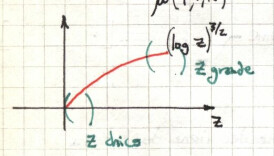
\includegraphics[scale=0.5]{images/1606329601.jpg}


La física del problema dependerá de (a) la dimensión del sistema (b) la relación $e(p)$. Notemos que por ejemplo
en 2D no hay condensación de Bose.

Sabíamos que 
\[
	U(z,V,T) = - \dpar{}{\beta}\log Q(z,V,T)
\]
\[
	U = \frac{3}{2} \frac{kT}{\lambda^3} f_{5/2}(z) = \frac{3}{2} PV
\]
y esto es válido para bosones, fermiones y boltzmanniones.

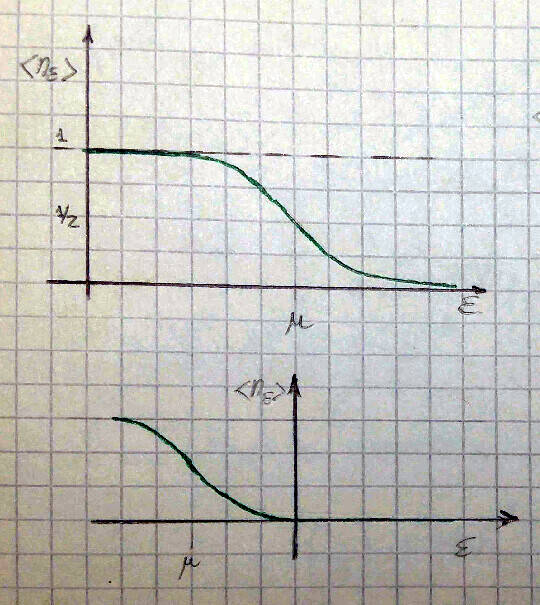
\includegraphics[scale=0.5]{images/1625624007.jpg}

\[
	\braket{n_e} = \frac{1}{z^{-1} \euler^{\beta e} + 1 } = \frac{1}{ \euler^{\beta ( \mu - e) } + 1 }
\]
Si $ \mu < 0 $ como $ e > 0 $ siempre, ni aún en el estado de más baja energía se llega a ocupar el
nivel (restan muchos niveles vacíos).

Sea que $ T \to \infty $ entonces $ \beta \to \infty $ y se sigue que 
\[
	\euler^{\beta(e-\mu)} \to \infty \qquad e> \mu
\]
\[
	\euler^{\beta(e-\mu)} \to 0 \qquad  e< \mu
\]
\[
	\euler^{\beta(e-\mu)} \to 1 \qquad  e = \mu
\]
Luego, con $ T = 0 $ es Fermi un escalón. El valor de $ \mu $ que determina el último
estado ocupado se llama $ e_F$ 


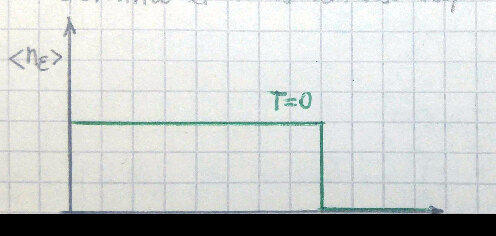
\includegraphics[scale=0.5]{images/1625624033.jpg}

\[
	f_{3/2}(z) = \frac{\lambda^3}{v} = \int_0^{\xi = \beta\mu } \frac{x^{1/2}}{\Gamma(3/2)3/2}dx =
	\frac{4}{3} \frac{1}{\pi^{1/2}} ( \beta\mu )^{3/2} = 
	\frac{4}{3} \frac{1}{\pi^{1/2}} ( \beta e_F )^{3/2}
\]

\notamargen{Pathria 132 cuentas de GC. Pathria 138 gases simples.}

% =================================================================================================
\subsection{Análisis del gas ideal de Fermi}
% =================================================================================================

La primera aproximación consiste en 
\begin{itemize}
 \item Caso no degenerado : $ \lambda^3 / v  \ll 1 $  que lleva a $ T $ alta y $ v $ alto
 por ende $ N/V $ chico (densidad baja).
 Es un gas diluído, el límite debería ir a Boltzmann (gas ideal clásico)
 \[	
	z \ll 1 \qquad f_\nu(z) \approx z \qquad \frac{\lambda^3}{v} \approx z
 \]
 Si vale la condición entonces 
 \[
	\frac{\lambda^3}{v} = \sum_{l=1}^\infty \frac{(-1)^{l+1} z^l }{l^{3/2}} 
	\sim z - \frac{z^2}{2^{3/2}} \ll 1 \qquad z \ll 1
 \]
 y vemos que se puede invertir para conseguir la expresión de $z$,
 \[
	z \sim \frac{\lambda^3}{V} + \frac{1}{2^{3/2}} \Frac{\lambda^3}{V}^2 \sim \frac{\lambda^3}{V} \ll 1
 \]
 y se tiene $ \euler^{\beta \mu} \ll 1$ y por ende $\mu \ll 0$. En el límite clásico $\mu \to -\infty$.
 \[
	\beta p V = \frac{v}{\lambda^3}\left( z - \frac{z^2}{2^{3/2}} + ... \right) \approx 
	1 + \frac{\lambda^3}{2^{5/2} v} \qquad \qquad 
	U = \frac{3}{2} \frac{N}{\beta}
	\left( 1 + \frac{\lambda^3}{2^{5/2} v} \right)
 \]
 \item $\frac{\lambda^3}{v} < 1 $ entonces $ z < 1 $ y hay que expandir el virial,
 \[
	\beta p V = \sum_{l=1}^\infty (-1)^{l-1} a_l \left(\frac{\lambda^3}{v} \right)^{l-1}
 \]
 que igualando coeficientes se hace (¿?)
 \notamargen{ $\lambda^3 / v $ a orden 1 hay efectos cuánticos }
 \[
	f_{5/2}(z) = f_{3/2}(z) \cdot \sum_{l=1}^\infty (-1)^{l-1} a_l \left(\frac{\lambda^3}{v} \right)^{l-1}
 \]
 \item $\frac{\lambda^3}{v} \approx 1 $ Cálculo numérico
 \item Caso altamente degenerado : $ \lambda^3 / v \gg 1 $ (bajas temperaturas y altas
 densidades), se tiene $ z \gg 1 $. 
 Se puede expandir $ f_\nu(z) $ en función de $ (\log )^{-1} $ mediante lema de Sommerfeld
 \notamargen{ $ z \ggg 1 $ entonces $ \log z \gg 1 $ $ ( \log z )^{-1} \ll 1 $ $ \log z = \beta \mu $ }
 \[
	f_{5/2}(z) = \frac{8}{15\pi^{1/2}} (\log z)^{5/2} \left[ 1 + \frac{5\pi^2}{8}(\log z)^{-2} + ... \right]
 \]
 \[
	f_{3/2}(z) = \frac{4}{3\pi^{1/2}} (\log z)^{3/2} \left[ 1 + \frac{\pi^2}{8}(\log z)^{-2} + ... \right]
 \]
 y entonces, tomando la más burda,
 \[
	\frac{\lambda^3}{v} = \frac{4}{3\pi^{1/2}} (\log z)^{3/2}  \quad \text{ a orden 0 }
 \]
 \[
	\frac{h^3}{ (2\pi mkT)^{3/2} } \frac{N}{V} \frac{3\pi^{1/2}}{4} (kT)^{3/2} = \mu^{ 3/2 }
 \]
 \[
	\frac{ h^3 }{ \pi } \frac{ N }{ V } \frac{ 3 }{ ( 2m )^{ 3/2 } 4 } = \mu^{ 3/2 } = e_F^{3/2}
 \]
 \[
	\frac{\lambda^3}{v}\frac{3\pi^{1/2}}{4} (kT)^{3/2} = 
	\mu^{3/2}\left[ 1 + \frac{\pi^2}{8}(\log z)^{-2} + ... \right]
 \]
 \[
	\frac{ h^3 }{ \pi } \frac{ N }{ V } \frac{ 3 }{ ( 2m )^{ 3/2 } 4 } = e_F^{3/2} \approx
	\mu^{3/2} \left[ 1 + \frac{\pi^2}{8}(\log z)^{-2} \right]
 \]
 \[
	e_F \approx \mu \left[ 1 + \frac{\pi^2}{8} \Frac{ \mu }{ kT }^{-2} \right]^{ 2/3 } \approx 
	\mu \left[ 1 + \frac{\pi^2}{12} \Frac{ kT }{ \mu }^{2} \right]
 \]
 \notamargen{Anoté {\it investigar este pasaje}. }
 
 Entonces si se tiene $0 < T \ll T_F$ resulta (realmente en la carpeta está al revés $\mu = e_F[]$, así
 que probablemente hay un cambio de signo y aproximaciones en el medio)
 )
 \[
	e_F \approx \mu \left[ 1 - \frac{\pi^2}{12}\Frac{ kT }{ e_F }^2 \right]
 \]
 y consideramos
 \[
	\frac{1}{\mu^2} \approx \frac{1}{e_F^2}
 \]
 pués $ \mu $ es muy grande.
 \[
	\beta p v = \frac{ f_{5/2}(z) }{ f_{3/2}(z) } \approx \frac{ 2 \beta \mu }{ 5 } 
	\left[ 1 + \frac{ 5\pi^2 }{ 8 } \left( \frac{kT}{\mu} \right)^2 \right]
	\left[ 1 - \frac{ \pi^2 }{ 8 } \left( \frac{kT}{\mu} \right)^2 \right]
 \]
 Hasta orden dos en $ T $ resulta 
 \[
	pv \approx \frac{ 2 \mu }{ 5 } \left[ 1 + \frac{ \pi^2 }{ 2 } \left( \frac{kT}{\mu} \right)^2 \right] =
	\frac{ 2 e_F }{ 5 }\left[ 1 - \frac{ \pi }{ 12 } \left( \frac{kT}{e_F} \right)^2 \right] 
	\left[ 1 + \frac{ \pi^2 }{ 2 } \left( \frac{kT}{e_F} \right)^2 \right] 
 \]
 \[
	pv \approx \frac{ 2 e_F }{ 5 } \left[ 1 + \frac{ 5 \pi^2 }{ 12 } \left( \frac{kT}{e_F} \right)^2 \right] 
 \]
 \[
	U = \frac{3}{2} p v \approx \frac{3}{5} N e_F 
	\left[ 1 + \frac{ 5 \pi^2 }{ 12 } \left( \frac{kT}{e_F} \right)^2 \right] 
 \]
 \[
	C_V = \dpar{U}{T} \approx \frac{ N \pi^2 k^2 T }{ 2e_F } \qquad C_V \propto T
 \]
 \[
% 	C_V \approx \frac{\pi^2}{2} Nk \left( \frac{T}{T_F} \right)
	C_V \approx \frac{\pi^2}{2} Nk \Frac{T}{T_F}
 \]
 DIBUJO 
 $T_F$ siempre estará en general en la zona clásica donde no vale la aproximación degenerada.
 
 Calor específico Fermi (¿?) se anula con $ T = 0 $
 
 Tomé notas de una evaluación más
 \[
	f_{11/2}(z) \approx \frac{2}{\sqrt{\pi}}(\log z)^{1/2} \left[ 1 - \frac{\pi^2}{24}(\log z)^{-2} + ... \right]
 \]
 que harían llegar a una corrección (notar que arriba fui hasta orden cero nomás)
 \[
	\frac{\lambda^3}{V} \sim \frac{4}{3\sqrt{\pi}} (\log z)^{3/2} \left[ 1 - \frac{\pi}{8}(\log z) \right]
 \]
 
 Otra cosa es la integral
 \[
	N = \int_0^\infty \: g(e) n_e \: de \longrightarrow 
	\int_0^\infty \: \frac{g(e)}{ \euler^{\beta(e-\mu)+1}} de
 \]
 y vemos que la dimensionalidad entra en $g(e)$ mientras el denominador va al escalón con temperatura nula.
 En este último caso la integral es $\int^{e_F} g(e) \: de$. Pero para $T \sim 0$ la itnegral es más complicada
 y el lema de Sommerfeld ayuda,

 \begin{multline*}
	\int_0^\infty \: \frac{\phi(x)}{ \euler^{x-\xi} + 1} dx = 
	\int_0^\xi \: \phi(x) \: dx + \frac{\pi^2}{6} \dtote{\phi}{x}{x=\xi}  +\\
	\frac{7\pi^4}{360} \dtote[3]{\phi}{x}{x=\xi}  + \frac{31\pi^5}{15120} \dtote[5]{\phi}{x}{x=\xi} 
 \end{multline*}

 \item Caso totalmente degenerado : $\frac{\lambda^3}{v} \to \infty \qquad (T \to 0) \qquad z \to \infty $
 
 La distribución de estados es escalón,
 \[
	\braket{N} = \frac{ 4 \pi V }{ h^3 } \int_0^{p_F} p^2 \Frac{ 1 }{ z^{-1} \euler^{\beta p^2 / 2m } + 1} dp
 \]
 \notamargen{$ z = \euler^{\beta\mu} $ y $z(T\to 0) = \euler^{\beta e_F } \to \infty $}
 \[
	\braket{N} = \frac{ 4 \pi V }{ h^3 } \int_0^{p_F} p^2 dp
 \]
 
 Notemos que 
 \notamargen{Teniendo el límite sale la cuenta}
 \[
	pV = \frac{ 4 \pi V }{ h^3 } \int_0^{p_F} p^2 kT \log (1 + \euler^{ -1/kT( p^2/2m - \mu_0 )} ) dp
 \]
 tiene un comportamiento no trivial con $ T \to 0 $. Si $ kT \to 0 $ entonces si $e > \mu_0$ el $\log \to 0$
 y si $e < \mu_0$ el $\log \to \infty $.
 Parecería que con $ T \to 0 $ es
 \[
 	pV = \frac{ 4 \pi V }{ h^3 } \int_0^{p_F} p^2 \left( \frac{ p^2 }{ 2m } - \mu_0 \right) dp
 \]
 y haciendo el cambio de variables de acuerdo a $ p^2 / 2m = e $, que lleva a $ pdp = m de $, se tiene 
 \[
 	pV = \frac{ 4 \pi V }{ h^3 } \int_0^{e_F} \sqrt{2e} m^{3/2} ( e -\mu_0 ) de
 \]
 \[
	pV = \frac{ 4 \pi V }{ h^3 } 2^{ 1/2 } m^{ 3/2 } 
	\left( \frac{e_F^{ 5/2 }}{5/2} - \mu_0 \frac{e_F^{ 5/2 }}{3/2} \right) =
	\frac{ 4 \pi V }{ h^3 }2^{ 1/2 } m^{ 3/2 } e_F^{ 5/2 } \frac{ 4 }{ 15 }
 \]
 \[
	U = \frac{3}{2} p V = \frac{ 4 \pi V }{ h^3 }2^{ 1/2 } m^{ 3/2 } e_F^{ 5/2 } \frac{ 2 }{ 5 }
 \]
 \[
	p = \frac{2}{5} e_F \frac{\braket{N}}{V} \qquad U = \frac{3}{5} e_F \braket{N} 
 \]
 A $ T = 0 $ tenemos presión y energía no nulas; las partículas no se acomodan todas en un único nivel energético
 (exclusión de Pauli).
 Para $ T \approx 0 $ ( $T$ bajas) el escalón en estados apenas se desdibuja

 
 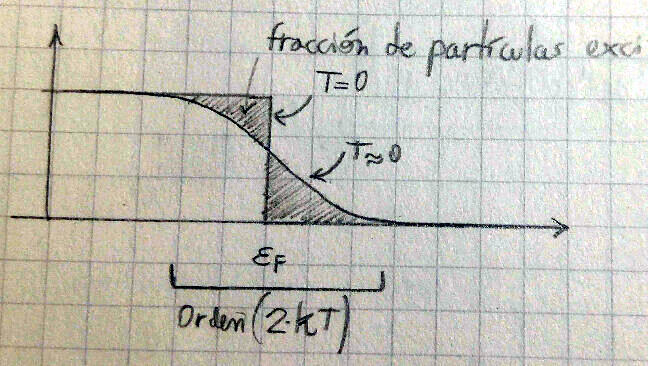
\includegraphics[scale=0.4]{images/1625624063.jpg}
 
\end{itemize}

En relación a esto último tenía el límite $ T \to 0 $ para la densidad de estados,
\[
	\vm{n_e} = \frac{ 1 }{ z^{-1}\euler^{\beta e} + 1 } = 
	\frac{ 1 }{ \euler^{\beta (e-\mu)} + 1 } \quad T \to 0 \quad 
	\begin{cases}
		1 \quad e < \mu (T=0) \\
		0 \quad e > \mu (T=0) 
	\end{cases}
\]
y vemos que la cosa depende del signo de $(e - \mu)$ y  $ \sum_e \vm{n_e} = N $, pero
en el continuo

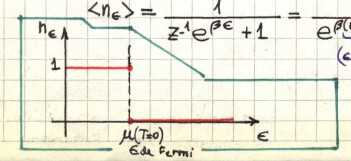
\includegraphics[scale=0.5]{images/1606329575.jpg}

\[
	 \sum_e \vm{n_e} = N \qquad \longrightarrow \int_0^\infty \: g(e) n_e \: de = N
\]
pero si tenemos el valor de la energia de Fermi basta integrar hasta allí,
\[
	\int_0^{e_F} \: g(e) n_e \: de = N
\]
donde $de \: g(e)$ dependerá de la relación entre $E$ y $p$ y la dimensión del problema.

Podemos definir una presión y energía de Fermi así
\[
	e_F = \frac{p_f^2}{2m} \qquad \qquad e_F = k T_F
\]
con un gas que tiene $ T < T_F $ es un gas altamente degenerado y será
\[
	e_F = \frac{ \hbar^2 }{ 2 m } \Frac{ 6 \pi^2 }{ v }^{3/2}
\]
Ahora bien, si las partículas tienen spin entonces es $g=2$ de modo que
\[
	\int_0^{e_F} de g g(e) = N
\]
en este caso será más chica la energía de Fermi. 
Veamos qué pasa a temperaturas bajas con $C_V$ y $U$.
Para los números de ocupación se tiene el gráfico bajo estas lineas

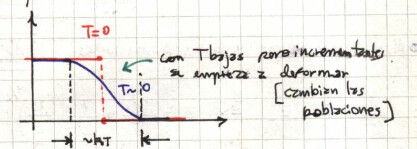
\includegraphics[scale=0.5]{images/1606329581.jpg}

Luego será
\[
	U = \sum_e \: e n_e = \frac{3}{5} N e_F \left[ 1 + \frac{5\pi^2}{12}\Frac{kT}{e_F}^2 + ... \right]
\]
y entonces tendremos

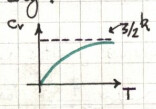
\includegraphics[scale=0.5]{images/1606329585.jpg}

Para la presión es $ P(T=0) = 2/3 U(T=0)/V$ pero como $ U = 3/5 N e_F $,
hay presión porque al ser ferminones igualmente hay cierta repulsiçon: la visión clásica de $T=0$ con
partículas quietas no es apropiada.

El número de partículas excitados puede venir de $ \sim N k T / e_F $ entonces estando relacionado
con al análogo del $kT$. El Pathria comenta esto en pag. 199.


\begin{ejemplo}{\bf Problema 4}

Gas de electrones 2D. Altamente degenerado, entonces la temperatura está en $ 0 < T \ll T_C $.
Se puede partir desde
\[
	\vm{E} = P A
\]
y vemos que vale en general para $D$ dimensiones
\[
	P L^D = \frac{ 2 }{ D } \vm{ E }
\]
y luego
\[
	\frac{ P A }{ k T } = \log Z_{GC} = 2 \sum_p \: \log ( 1 + z \euler^{-\beta e_P})
\]
donde el primer dos está asociado al spin. En el paso al continuo resulta
\[
	\frac{ P A }{ k T } = \frac{ 2 A}{h^3} \int 2 \pi dp \log ( 1 + z \euler^{-\beta e_P}) 
\]
o bien
\[
	\frac{4 \pi A m}{h^2} \left( \left. e \log ( 1 + z \euler^{-\beta e_P} ) \right|_0^\infty + 
	\beta \int \frac{ e \: de }{\euler^{\beta(e-\mu)}+1} \right)
\]
donde se ve que el primer término desaparece y entonces si es $T=0$ basta integrar hasta la energía 
de Fermi y con $T\sim 0$ hay que usar el lema de Sommerfeld, en cuyo caso tenemos
\[
	\frac{4 \pi A m}{h^2} \left( \frac{ \beta \mu^2 }{ 2 } + \frac{ \pi^2 }{ 6 \beta } \right)
\]
de manera que finalmente
\[
	\vm{E} = \frac{4 \pi A m \mu^2 }{2h^2} \left( 1 + \frac{ \pi^2 }{ 3 \mu^2 }(kT)^2 \right).
\]
\end{ejemplo}


\begin{ejemplo}{\bf Problema 5}

Tenemos electrones en presencia de un campo $\vb{H}$. El spin interactuará con el campo y será
\[
	\frac{ p^2 }{ 2 m } + s \: \mu_B H
\]
donde $s=-1$ implica que el spin está paralelo al campo y $s=+1$ implica que está antiparalelo

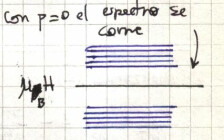
\includegraphics[scale=0.5]{images/1606329613.jpg}

A una temperatura $T=0$ el estado minimiza $F=U-TS$ de manera que $F=U$ pero para $T\sim 0$ el 
estado minimizará con un compromiso entre U y S por las combinaciones posibles

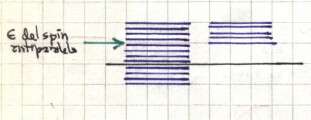
\includegraphics[scale=0.5]{images/1606329617.jpg}

La $e_F = \mu_B H$ para que todos se hallen paralelos al campo. De aquí surge una relación entre
la densidad y la energía. Entonces
\[
	n_+ = \frac{ 1 }{ \euler^{ \beta( p^2/(2m) + s \: \mu_B H - \mu } + 1 } \qquad \qquad 
	n_- = \frac{ 1 }{ \euler^{ \beta( p^2/(2m) - s \: \mu_B H - \mu } + 1 }
\]
e integrando llevo a $N_+ + N_- = N$. Serán $M = \mu_B( N_+ - N_- ) $ y luego será
\[
	\chi = \lim_{H\to 0} \Frac{M}{H}
\]
si este límite es positivo tendremos paramagnetismo, magnetización proveniente del acople entre
el campo y el spin mientras que si es negativo tendremos diamagnetismo, magnetización proveniente
del acople del momento angular orbital con el campo.

\end{ejemplo}

{\bf Comentario suelto}: metal se puede pensar como un sólido elástico más un gas de electrones. 
Un fonon es una excitación en la red.

% =================================================================================================
\section{Cuánticos III --reubicar--}
% =================================================================================================
 
 \subsection{Los números de ocupación}
 
 
 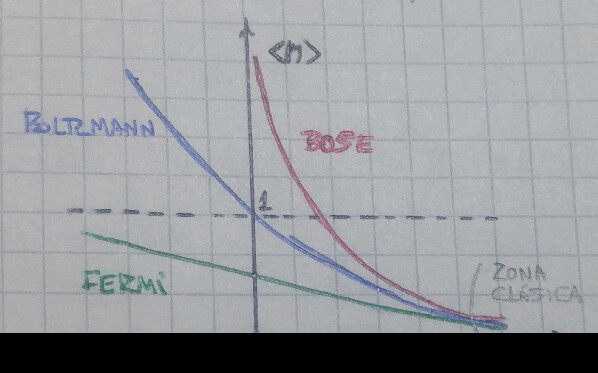
\includegraphics[scale=0.4]{images/1625624267.jpg}
 
 Se ve que para Bose $ \mu < 0 $ siempre pero $ \braket{n} \to \infty $ si $ \mu \to 0^+ $.
 El gráfico es para $T$ alta. Con $ T $ bajas todo tiende a suceder más pegado al eje $ \beta(e-\mu) = 0 $
 
 \subsection{Comportamiento de $ f_{3/2}(z) $}
 
 \[
	f_{3/2}(z) = \sum_{j=1}^\infty (-1)^{j+1}\frac{z^j}{j^{3/2}} \approx z - \frac{z^2}{2^{3/2}} \qquad 
	\text{ $z$ chico }
 \]
 \[
 	f_{3/2}(z) = \frac{1}{\Gamma(3/2)} \int_0^\infty \frac{x^{1/2}}{z^{-1}\euler^{x} + 1} dx \approx  
 	\frac{1}{\Gamma(3/2)} \int_0^{\log z = \beta\mu} x^{1/2} dx
 \]
 
Notemos que con $ \beta \mu $ grande el integrando es 1 o 0 (DIBUJO); en realidad es un escalón en el límite
en que $ \xi \equiv \beta\mu \to \infty$
\notamargen{Definimos $ \log z \equiv \xi $ para no especular con temperaturas. }

\[
	f_{3/2}(z) = \frac{4}{ 3 \sqrt{\pi} } (\log z )^{3/2} \text{ $z$ muy alto }
\]
\[
	f_{3/2}(z) = \frac{4}{ 3 \sqrt{\pi} } \left[ (\log z )^{3/2} + \frac{\pi^2}{8}(\log z )^{-1/2} + ... \right]
\]

El valor $ \lambda^3 / v $ determina relación entre $ T,V,N $ que son los parámetros macroscópicos que uno fija.

\subsection{Casos}

\begin{itemize}
 \item Comportamiento clásico: $\frac{\lambda^3}{v} \ll 1$ Altas $T$ y bajas $n\equiv \frac{N}{V}$ 
 \[
	\frac{\lambda^3}{v} = f_{3/2}(z) \approx z - \frac{z^2}{2^{3/2}}
 \]
 y por inversión de la serie 
 \[
	z = \frac{\lambda^3}{v} + \Frac{\lambda^3}{v}^2 2^{-3/2}
 \]
 \notamargen{Sabemos que en Boltzmann es $\frac{\lambda^3}{v} = z$ }
 y entonces si $\frac{\lambda^3}{v} \ll 1$ se tiene que $ z \ll 1 $
 \[
	\frac{pv}{kT} = \frac{v}{\lambda^3} f_{5/2}(z) \qquad \qquad \frac{\lambda^3}{v} = f_{3/2}(z)
 \]
 \[
	\frac{pv}{kT} = \frac{f_{5/2}(z)}{f_{3/2}(z)} \approx \frac{z - z^2/2^{5/2}}{z - z^2/2^{3/2}}
	\approx 1 + \frac{1}{2^{3/2}} \Frac{\lambda^3}{v}
 \]
 siendo el último término una corrección cuántica.
 
  \item Comportamiento cuántico : $\frac{\lambda^3}{v} \gg 1$ Bajas $T$ y altas $n\equiv \frac{N}{V}$ 
  
  A $ T = 0 $ determinamos la $ e_F $ como (con el límite de $T\to 0$)
  \[
	\frac{\lambda^3}{v} = \frac{1}{\Gamma(3/2)} \int_0^{\log z = \beta\mu} x^{1/2} dx = 
	 \frac{4}{ 3 \sqrt{\pi} } (\log z )^{3/2}
  \]
  \[
	\Frac{ 3  \lambda^3  \sqrt{\pi} }{4v}^{2/3} = \Frac{ 3  h^3  \sqrt{\pi} }{4(2\pi m k T)^{3/2}v}^{2/3} 
	= \log z =  \beta e_F
  \]
  \[
	\frac{h^2}{2m}\Frac{3}{4\pi v}^{2/3} = e_F = \frac{\hbar}{2m}\Frac{6\pi^2}{v}^{2/3}
  \]
  A $ T = 0 $ la ocupación por nivel es un escalón ($e_F = \mu(T=0) $) 
  \[
	\braket{n_e} = 	\begin{cases}
			1 \qquad e < e_F \\
			0 \qquad e > e_F
			\end{cases}
  \]
  Estoy ya lo grafiqué antes. Hay que consolidar todo este material.
\end{itemize}

\subsection{Funciones termodinámicas con $T$ baja y $n$ alta}

Usamos Sommerfeld
\[
	\frac{\lambda^3}{v} = f_{3/2}(z) \qquad  \qquad \mu = e_F
\]
orden 1
\[
	\frac{\lambda^3}{v} =  
	\frac{4}{3\sqrt{\pi} } (\log z )^{3/2} \left[ 1 + \frac{\pi^2}{8}(\log z )^{-2} \right] 
\]
\[
	\frac{\lambda^3}{v} \frac{3\sqrt{\pi} }{4} \left[ 1 + \frac{\pi^2}{8}(\log z )^{-2} \right]^{-1} 
	\approx (\log z)^{3/2} 
\]
\[
	e_F \left( 1- \frac{\pi^2}{12}\Frac{T}{T_F}^2 \right) \approx \mu( T ) \text{ cumple $\mu(T=0)=e_F$}
\]
Puede verse que con $ \frac{\lambda^3}{v} \ggg 1 $ ($T$ baja y $n$ alta) es
\[
	C_V \approx \frac{N \pi^2 k^2 T}{2 e_F}
\]
DIBUJO

Aún a $T=0$ hay presión no nula pero $S \to 0$ con $T \to 0$ respetando la tercera ley.
Existe una relación de recurrencia
\[
	z\dpar{}{z} f_\nu(z) = z\dpar{}{z} \sum_{l=1}^\infty (-1)^{l+1} \frac{z^l}{l^\nu} =
	\sum_{l=1}^\infty (-1)^{l+1} \frac{l z^{l-1} z}{l^\nu} = 
	\sum_{l=1}^\infty (-1)^{l+1} \frac{z^l}{l^{\nu-1}} = f_{\nu-1}(z)
\]
\[
	f_\nu(z) = \int \frac{1}{z} f_{\nu-1}(z) dz
\]
\[
	f_{3/2}(z) \approx \frac{4}{3\sqrt{\pi}} (\log z)^{5/2}
\]
entonces
\[
	f_{5/2}(z) = \int dz \frac{4}{3\sqrt{\pi}} \frac{(\log z)^{3/2}}{z} =
	 \frac{4}{3\sqrt{\pi}} \int dz \frac{ 2 }{ 5 } \dpar{}{z} (\log z)^{5/2} =
	\frac{8}{15\sqrt{\pi}}(\log z)^{5/2}
\]
\notamargen{Usamos $d(\log z)^n = n (\log z)^{n-1}/z $}

\subsection{Sobre la aproximación de gas de Fermi para el núcleo}

En lo que sigue una deducción más detallada del cálculo.
Considero una caja de lados $L$
\[
	\vb{k} = \frac{2\pi}{L} \vb{n} \qquad \hbar \vb{k} = \vb{p} = \frac{h}{L} \vb{n}
\]
\notamargen{Tomo en el origen de coordenadas $n_i = \pm 1, \pm 2, ...$ y así voy de $-L/2$ a $L/2<$.}
\[
	E = \frac{( \hbar |\vb{k}| )^2}{ 2m } = \frac{ \hbar^2 }{ m } \frac{2\pi^2}{L^2}
	(n_x^2 + n_y^2 + n_z^2) \qquad n_i \in \mathbb{Z}
\]
Quiero saber qué densidad de estados energéticos tengo. Para ello, en esféricas
\[
	E = \frac{ \hbar^2 }{ m } \frac{2\pi^2}{L^2} r^2
\]
donde $r$ vive en la esfera (no es necesario tomar el octante y dividir sobre 8)
\[
	g(E) dE = N(r) dr = 4\pi r^2 dr
\]
siendo $g(E) dE$ el número de puntos entre $E$ y $E+dE$,
\[
	dE = \frac{(\hbar \pi)^2}{L^2 m}4 r dr 
\]
\[
	g(E) dE = \frac{ L^3 m^{3/2} E^{1/2} }{ \hbar^{3/2} \pi^2  \sqrt{2}}dE
\]
\[
	N = g\int_0^{e_F} g(E) dE = \sqrt{2} \frac{ V m^{3/2} }{ \hbar^3 \pi^2 } 
	\int_0^{e_F} e^{1/2} dE
\]
\[
	N = \frac{ V m^{3/2} }{ \hbar^3 \pi^2 } \frac{2^{3/2}}{3} e_F^{3/2}
\]
\[
	\frac{1}{v} = \frac{ m^{3/2} }{ \hbar^3 \pi^2 } \frac{2^{3/2}}{3} e_F^{3/2}
\]
y entonces deducimos de aquí que 
\[
	e_F = \frac{\hbar}{2m} \Frac{3\pi^2}{v}^{2/3}
\]
que coincide con la expresión para $e_F$ con degeneración $g=2$

\notamargen{¿Y estas cuentas sueltas?}
\[
	n_x^2 + n_y^2 + n_z^2 = r^2 \qquad V=\frac{4}{3}\pi r^3 \qquad dV = 4\pi r^2 dr
\]
\[
	E = \frac{(\hbar \pi)^2}{2ma^2}r^2 \qquad \qquad dE = \frac{(\hbar \pi)^2}{ma^2}r dr
\]
\[
	N(r) dr = \frac{\pi}{2} r^2 dr 
\]
será lo mismo que el incremento en niveles energéticos
\[
	N(e)de = \frac{m^2 a^3}{\pi^2 \hbar^3} \Frac{E}{2}^{1/2} dE
\]
Pensamos un conjunto de nucleones como un gas de Fermi. 
\notamargen{Recordemos que a $T=0$ era $pV=2/5 N e_F$ y $U=3/5 N e_F$}
Claramente
\[
	N = 2 \int_0^{e_F} N(e) \; de
\]
porque tenemos la ocupación en función de la energía
\[
	e_F \propto \Frac{N}{V}^{2/3} \text{ según la definición de $e_F$ }
\]

Al aplicar este modelo (del gas de Fermi) al núcleo hacemos algunas consideraciones
\[
	R = a_0 A^{1/3} \qquad V \propto A 
\]
siendo $A$ el número de nucleones.

Para un núcleo se tienen N=A-Z neutrones, siendo Z protones y A nucleones.
\[
	E = \frac{3}{5}N_Te_F (\text{ a } T=0)
\]
y tenemos un $e_F$ de protones y de neutrones, que son 
\[
	e_{Fp} \propto \Frac{Z}{A}^{2/3} \qquad \qquad 
	e_{Fn} \propto \Frac{A-Z}{A}^{2/3}
\]
\[
	E = \frac{3}{5}\left[ Z\Frac{Z}{V}^{2/3} + (A-Z)\Frac{A-Z}{V}^{2/3} \right] =
	\frac{3}{5}\Frac{ Z^{5/3} + (A-Z)^{5/3} }{A^{2/3}}
\]
donde hemos supuesto ambos pozos iguales. Si los pozos no fueran iguales cambia la
$e_F$.

Se minimiza $E$ con $Z=N=A/2$ (simetría)
\[
	f_4 \propto E-E_0 = \frac{3}{5A^{2/3}} \left[ Z^{5/3} + (A-Z)^{5/3} - 2(A/2)^{5/3} \right]
\]
que se puede reescribir en función de $D = (N-Z)/2 = (A - 2Z)/2 = A/2 - Z$ (que será chico) y
de esta manera 
\[
	Z = \frac{A}{2} - D \qquad A-Z = \frac{A}{2} + D
\]
\[
	f_4 \propto \frac{3}{5} \left( \frac{ [A/2 - D]^{5/3} + [A/2 + D]^{5/3} - 2[ A/2 ]^{5/3} }{A^{2/3}}\right)
\]
y que con un Taylor en $ D \approx 0 $ resulta 
\[
	f_4 \propto \frac{(A/2 - Z)^2}{A} \propto D^2 \text{ término de simetría }
\]

\subsection{Cuánticos 3 -- más material para reubicar--}

Un esquema de temas:
comportamiento de los números de ocupación
gas de Fermi : comportamiento de $f_\nu(z)$ con $ \nu = 3/2 $
gas de Fermi con condiciones extremas
\[
	\lambda^3 / v \ggg 1 \qquad \qquad \lambda^3 / v \lll 1
\]
$e_F$ con degeneración $g$
funciones termodinámicas con $\lambda^3 / v \ggg 1$ $ S \to 0 $ con $ T\to 0$
Aproximación de gas de Fermi para núcleo
densidad de estados $g(e)$


La expresión para $ \mu(T) $ con $ T \geq 0 $ sale de 
\[
	\frac{\lambda^3}{v} =  
	\frac{4}{3\sqrt{\pi} } (\log z )^{3/2} \left[ 1 + \frac{\pi^2}{8}(\log z )^{-2} \right] 
\]
\[
	( \log z )^{3/2} = \frac{ 3\sqrt{\pi} h^3 }{ ( 2 \pi m )^{3/2} (kT)^{3/2} 4v }   
	\frac{1}{\left[ 1 + \frac{\pi^2}{8}(\log z )^{-2} \right] }
\]
\[
	\mu = \Frac{3 \sqrt{\pi} }{4v}^{2/3} \frac{h^2}{2\pi m}
	\left( 1 + \frac{\pi^2}{8\log^2 z}\right)^{-2/3}
\]
\[
	\mu = e_F \left[ 1 - \frac{\pi^2}{12} \Frac{kT}{e_F}^2 \right]
\]
y con $T$ baja podemos escribir todo en función de la $e_F$.
\notamargen{Hay un yeite en la deducción que refiere a que abajo es lo mismo usar orden 1 que
orden dos y reemplazo $ (\beta \mu)^{-2} $ por $(\beta e_F)^{-2}$}
\[
	E = \frac{3}{5}Ne_F \qquad \qquad \text{ con } T=0
\]

Lo importante de tener $ f_{3/2}(z) $ en función de $ \lambda^3/v $, desde 
\[
	 \lambda^3/v  = f_{3/2}(z) 
\]
DIBUJO

es que vemos que $z$ chico lleva a $ \lambda^3/v $ grande y consecuentemente $z$ grande lleva a
$ \lambda^3/v $ grande.

Luego,
\begin{multline*}
	\text{ clásico } z \ll 1 \\
	\frac{ \lambda^3 }{ v } \ll 1 \text{ independientemente }
\end{multline*}
\begin{multline*}
	\text{ cuántico } z \gg 1 \\
	\frac{ \lambda^3 }{ v } \gg 1 \text{ independientemente }
\end{multline*}

Con $ T=0$ es $\mu(T=0)=e_F$
DIBUJO escalón

Cuántico (límite máximo) entonces
\[
	z \to \infty \Rightarrow \frac{ \lambda^3 }{ v } = \frac{4(\log z)^{3/2}}{3\sqrt{\pi}}
\]
\[
	\frac{ \lambda^3 }{ v } = \frac{4}{2\sqrt{\pi}}(\beta e_F)^{3/2} \text{ con } z=\euler^{\beta e_F}
\]

Entonces $e_F$ es el nivel tal que debajo de él hay N estados. En el espacio de momentos las partículas
ocupan una esfera de radio $p_F$.


\subsection{Estadísticas --otra cosa para reubicar--}

Esta sección es un sketchi

\[
	\braket{n}_i = \frac{1}{ \euler^{\beta(e_i - \mu)} + a} \qquad \qquad 
	\begin{cases}
	 a = 0 \quad \text{ MB } \\
	 a = -1 \quad \text{ BE } \\
	 a = 1 \quad \text{ FD } 
	\end{cases}
\]

DIBUJO 

Graficamos $1/ \euler^x + a $
En la zona clásica coinciden las tres y es
\[
	\euler^{\beta (e_i - \mu)} \gg 1 \forall e_i \; \text{ de interés }
\]
\[
	z^{-1} \euler^{\beta e_i } \gg 1 \qquad \qquad \beta(e_i - \mu) \gg 0
\]
\[
	\euler^{\beta e_i } \gg z \qquad \qquad e_i \gg \mu
\]
de (2) se deduce que como $e_i$ pueden ser $\approx 0$ entonces $0\gg\mu$ y por lo tanto
$\euler^{\beta\mu} \equiv z \ll 1$ de (1)
\[
	1 \gg \euler^{\beta\mu} \qquad \qquad 0 \gg \beta\mu
\]

Clásicamente $\euler^{\beta\mu}$ domina sobre $z$
\[
	\mu < 0 \text{ y } |\mu| \gg 1 
\]
\[
	\text{ Bose } \mu < \text{ todo } e
\]
\[
	\text{ Fermi } \mu \text{ sin restricción }
\]


Para $ z \ggg 1 $ conviene definir $ \xi = \log z $ y entonces 
\[
	f_\nu(z) = \frac{1}{\Gamma(\nu)} \int_0^\infty \frac{x^{\nu-1}}{\euler^{x-\xi}+1} dx
\]

Siendo $\xi$ grande se tendrá que 
\[
	F = \frac{ 1 }{ \euler^{x-\xi} + 1 } = \begin{cases}
	                  1 \qquad x < \xi \\
	                  1/2 \qquad x=\xi \\
	                  0 \qquad z > \xi
	                 \end{cases}
\]
En este supuesto $ \xi \ggg 1 $ podemos integrar
\[
	f_\nu(z) \approx \frac{1}{\Gamma(\nu)} \int_0^\infty x^{\nu-1} dx
\]
donde suponemos $ T \gtrsim 0 $ con lo cual $ \beta\mu \to \infty, \xi \to \infty$ y 
$z^{-1} \to 0, \euler^{-\xi} \to 0$

\[
	f_\nu(z) \approx \frac{ \xi^\nu }{\Gamma(\nu) \nu}
\]

Con $ \nu = 3/2 $ resulta 
\[
	f_{3/2}(z) \approx \frac{ (\log z)^{3/2} }{\Gamma(3/2) 3/2}
\]
\[
	\frac{\lambda^3}{v} = \frac{4}{3} \frac{1}{\pi^{1/2}}(\beta\mu)^{3/2} \to
	\left( f_{3/2}(z) \frac{3\sqrt{\pi}}{4}\right)^{2/3} \frac{1}{\beta} = e_F
\]
\[
	\frac{h^2}{2m} \Frac{3}{4v\pi}^{2/3} = \mu = e_F (\mu \text{ a } T=0 )
\]

La $e_F (\mu \text{ a } T=0 )$ es la energía hasta la cual se hallan ocupados los
niveles energéticos. Con $ T \gtrsim 0$ la ocupación es un escalón

DIBUJO 

La $e_F$ es el valor de $\mu (T=0)$

La energía $U$ es 
\[
	U  = \frac{3}{2} p V = \frac{3V}{2\beta\lambda^3} f_{3/2}(z) = \frac{3N}{2\beta} \frac{f_{5/2}(z)}{f_{3/2}(z)}
\]

Tenemos una aproximación de Sommerfeld para $z$ grande 
\[
	f_{3/2}(z) = \frac{ 4 }{ 3\sqrt{\pi} } (\log z)^{3/2} \left[ 1 + \frac{\pi^2}{8}(\log z)^{-2} + ... \right]
\]
\[
	f_{5/2}(z) = \frac{ 8 }{ 15\sqrt{\pi} } (\log z)^{5/2} \left[ 1 + \frac{5\pi^2}{8}(\log z)^{-2} + ... \right]
\]
\[
	U = \frac{ 3N }{ 5\beta } (\log z) 
	\left[ 1 + \frac{5\pi^2}{8}(\log z)^{-2} + ... \right]
	\left[ 1 + \frac{\pi^2}{8}(\log z)^{-2} + ... \right]^{-1}
\]
\[
	U = \frac{3\mu}{5} \left[ 1 + \frac{5\pi^2}{8}(\log z)^{-2} + ... \right] =
	\frac{3\mu}{5} + \frac{15\pi^2\mu}{60} \Frac{1}{\beta\mu}^2 + ...
\]
\[
	C_v \equiv \dpar{}{T}U/N \cong \frac{\pi^2}{2} \frac{k^2 T}{\mu}
\]
entonces con $T \gtrsim 0$ es $C_v \propto T$ y con $T=0$ es
\[
	\frac{ U}{N} = \frac{3}{5} e_F
\]
\[
	\frac{ U}{N} = \frac{3}{5} e_F \left( 1 + \frac{5\pi^2}{12} 
	\Frac{T}{\underbrace{e_F/k}_{\equiv T_F}}^2 + ... \right) 
\]

Para $z \approx 1$ se debe expandir en el virial
\[
	\frac{pV}{NkT} = \sum_{l=1}^\infty a_l \Frac{\lambda^3}{gv}^{l-1} (-1)^{l-1}
\]

Sabemos que 
\[
	\frac{p}{kT} = \frac{f_{5/2(z)}}{\lambda^3}
\]
y entonces con las expresiones de $f_\nu$,
\[
	\frac{pV}{NkT} = \frac{ \sum_{j=1}^\infty (-1)^{j+1} z^j / j^{5/2} }
	{ \sum_{k=1}^\infty (-1)^{k+1} z^k / k^{3/2} }
\]

Debemos usar toda la serie 
\[
	\left[ \sum_{l=1}^\infty a_l \Frac{\lambda^3}{gv}^{l-1} (-1)^{l-1} \right]
	\left[ \sum_{k=1}^\infty (-1)^{k+1} z^k / k^{3/2} \right] =
	\sum_{j=1}^\infty (-1)^{j+1} z^j / j^{5/2}
\]

Resultan
\[
	\begin{cases}
	 a_1 = 1 \\
	 a_2 = -0.17678 \\
	 a_3 = -0.00330
	\end{cases}
\]
\[
	\frac{pV}{NkT} = 1 + 0.17678 \underbrace{\Frac{\lambda^3}{gv}}_{\propto T^{-3/2}} 
	- 0.00330\Frac{\lambda^3}{gv}^2
\]

Usando 
\[
	U = 3/2 p V
\]
\[
	\frac{U}{N} \cong 3/2 kT \left( 1 + 0.17678 \Frac{\lambda^3}{gv} \right)
\]
\[
	\dpar{}{T} \frac{U}{N} = C_v = 3/2 kT \left( 1 + 0.17678 \Frac{\lambda^3}{gv} \right)
	+ \frac{3}{2} kT 0.17678 \frac{h^3}{gv(2\pi mk)^{3/2}2/3 T^{5/2}}
\]
y se puede despejar
\[
	c_v = \frac{3}{2} k \left[ 1- 0.08839 \Frac{\lambda^3}{gv}  \right]
\]

% =================================================================================================
\section{Estudio de un metal -- título tentativo --}
% =================================================================================================

\subsection{Estudio de un metal}

Modelamos un metal como una red de átomos que pueden oscilar y un gas de electrones
\[
	(\vb{x}_1, ...,\vb{x}_N ) \qquad \qquad \text{ $N$ átomos }
\]
\[
	(\vb{x}_1^0, ...,\vb{x}_N^0 ) \qquad \qquad \text{ Equilibrio fundamental }
\]


 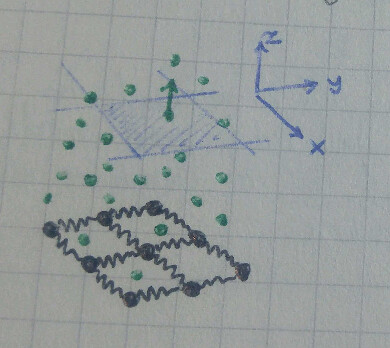
\includegraphics[scale=0.5]{images/1625625370.jpg}

Los desplazamientos del equilibrio serán 
\[
	\vb{x}_i - \vb{x}_i^0 = \vec{\xi}_i
\]
\notamargen{Planteo de un potencial de pequeñas oscilaciones}
\[
	K = \sum_i \frac{m}{2} | \vec{\xi}_i|^2 \qquad \text{ cinética }
\]
\[
	V = V(\{ \vb{x}_i^0 \}) + \sum_i \underbrace{\left. \dpar{V}{\vb{x}_i}\right|_{\vb{x}_i}}_{=0}
	(\vb{x}_i-\vb{x}_i^0) + 
	\sum_{i,j} \frac{1}{2} \dpar{V}{\vb{x}_i}{\vb{x}_j} (\vb{x}_i-\vb{x}_i^0) (\vb{x}_j-\vb{x}_j^0)
\]
\notamargen{Es cero porque está evaluado en el mínimo.}
\[
	V = V_0 + \sum_{i,j} \frac{1}{2} k_{ij}  \vec{\xi}_i\cdot  \vec{\xi}_j \qquad \text{ potencial }
\]
siendo las constantes de fuerza $k_{ij}$ las que controlan la interacción 
\[
	H = V_0 + \frac{m}{2} | \vec{\xi}_i|^2  + \sum_{i,j} \frac{1}{2} k_{ij}  \vec{\xi}_i\cdot  \vec{\xi}_j
\]

Este hamiltoniano se puede pasar a modos normales diagonalizando la matriz de fuerzas
\[
	H = V_0 + \frac{m}{2}  \sum_i^{3N} \left( \dot{q}_i^2 + \omega_i^2 q_i^2 \right)
\]
y $\omega_i$ son las frecuencias de los $3N$ modos normales del sistema de $N$ grados de libertad en
3D. En modos normales el hamiltoniano del sistema es el de $3N$ osciladores armónicos independientes
(no acoplados. 
Puede resolverse mediante los operadores de bajada y de subida (cuántica) resultando en
\[
	E = \sum_i^{3N} \left( n_i + \frac{1}{2} \right) \hbar \omega_i
\]
donde $n_i$ es el número de fonones (ocupación) del modo normal $i-$ésimo.

Estos fonones, cuasipartículas, son bosones porque pueden ser 
\[
	n_i = 0,1,2,...,\infty
\]
y su número total no está fijo ($\mu=0$ pues la energía no depende del número de fonones)
\[
	n_i = \frac{1}{\euler^{\beta\hbar \omega_i} -1 }
\]
pues $\hbar\omega_i$ es la energía del estado $i-$ésimo
\[
	n_i = \frac{1}{\euler^{ \hbar \omega_i / kT } -1 }
\]
\[
	E = V_0 + \frac{1}{2} \sum_i^{3N} \hbar \omega_i + \sum_i^{3N} n_i \hbar \omega_i
\]

La función de partición canónica será 
\[
	Q = \sum_E \euler^{ -\beta E } =
	\sum_E \euler^{ -\beta \left( \frac{1}{2} \sum \hbar \omega_i + \sum n_i \hbar \omega_i \right) }
\]
\[
	Q = \sum_{n_1=0}^\infty \sum_{n_2=0}^\infty ... \sum_{n_N=0}^\infty 
	\euler^{ -\beta \sum \left( \hbar \omega_i /2  + n_i \hbar \omega_i \right) }
\]
\[
	Q = \sum_{n_1} \euler^{ -\beta \left( \hbar \omega_1 /2 + n_1 \hbar\omega_1 \right) }
	\sum_{n_2} \euler^{ -\beta \left( \hbar \omega_2 /2 + n_2 \hbar\omega_2 \right) } \; ...
\]
\[
	Q = \prod_i^{3N} \left(
	\sum_{n_i=0} \euler^{ -\beta \left( \hbar \omega_i /2 + n_i \hbar\omega_i \right) } 
	\right) = \prod_i^{3N} \left(
	\sum_{n_i=0} \euler^{ -\beta n_i \hbar\omega_i } \right) \euler^{ -\beta \hbar \omega_i /2 }
\]
\[
	Q = \prod_i^{3N} \left(
	\frac{1}{1-\euler^{ -\beta \hbar \omega_i } } \right)  \euler^{ -\beta \hbar \omega_i /2 } = 
	\prod_i^{3N} \left( \frac{1}{ \euler^{ \beta \hbar \omega_i } -\euler^{ -\beta \hbar \omega_i } } \right)
\]
\[
	\log Q = \sum_i^{3N} \log \left( \frac{1}{ \euler^{ \beta \hbar \omega_i } -\euler^{ -\beta \hbar \omega_i } } 
	\right) = 
	\sum_i^{3N} - \log \left( { \euler^{ \beta \hbar \omega_i } -\euler^{ -\beta \hbar \omega_i } } \right)
\]
\[
	\log Q = \sum_i^{3N} - \log \left( 2 \sinh \Frac{\hbar\omega_i}{2kT} \right)
\]

Si quisiéramos pasar al continuo resultaría (con $N \to \infty$)
\[
	\log Q = - \int_0^\infty d\omega g(\omega) \log \left[ 2 \sinh \Frac{\beta\hbar\omega_i}{2} \right]
\]
donde $ g(\omega) $ es la densidad de estados y 
\[
	d\omega g(\omega) = \text{ \# de modos normales con frecuencia entre $\omega$ y $\omega + d\omega$ }
\]

Tenemos dos métodos de cálculo de energía
\begin{center}
\begin{tabular}{l|l}
$ \displaystyle E = \sum_i^{3N} ( n_i + 1/2 )\hbar\omega_i $ & 
$ \displaystyle -\dpar{\log Q}{\beta} = \sum_i^{3N} \frac{1}{\euler^\Box - \euler^{-\Box}}( \euler^\Box + 
\euler^{-\Box} )\frac{\hbar\omega_i}{2} $ \\
& \\
$ \displaystyle \sum_i^{3N} \hbar\omega_i\Frac{1/2\euler^{\beta\hbar\omega_i}+1/2}{\euler^{\beta\hbar\omega_i}-1} $  & 
$ \displaystyle -\dpar{\log Q}{\beta} = \sum_i^{3N} \Frac{\euler^\Box + \euler^{-\Box}} {\euler^\Box - \euler^{-\Box}} 
\frac{\hbar\omega_i}{2} $ \\
& \\
$ \displaystyle \sum_i^{3N} \frac{\hbar\omega_i}{2}\Frac{\euler^{\beta\hbar\omega_i}+1}{\euler^{\beta\hbar\omega_i}-1} $ 
& $ \displaystyle = \sum_i^{3N} \Frac{\euler^{2\Box} + 1 }{ \euler^{2\Box} - 1 } \frac{\hbar\omega_i}{2} $ \\
\end{tabular}
\end{center}

Por supuesto ambas coinciden. Observemos que 
\[
	\text{ \# de fonones } = \sum_i^{3N} n_i
\]
es una cantidad que no es fija (se crean y se destruyen). Por ello podemos evaluar fácilmente el
$Q$.

Desde $E$ se puede evaluar el $C_v$
\[
	\dpar{E}{T} = \sum_i^{3N} \frac{\hbar\omega_i}{2} \dpar{}{T}\Frac{ \cosh \Box }{ \sinh \Box } 
\]
\[
	C_v = \sum_i^{3N} \frac{\hbar\omega_i}{2} \left[ 
	\frac{ \sinh \Box }{ \sinh \Box }\dpar{\Box}{T} - \frac{ \cosh^2 \Box }{ \sinh^2 \Box } \dpar{\Box}{T}
	\right]
\]
\[
	C_v = \sum_i^{3N} \frac{\hbar\omega_i}{2}  \frac{\hbar\omega_i}{2k} \Frac{-1}{T^2} 
	\Frac{-1}{\sinh^2 \Box}
\]

Tenemos el modelo de Einstein, que usa $ \omega_i = \omega_E \forall i $ y entonces 
\[
	C_v = 3N k \Frac{\hbar\omega_E}{kT}^2 \frac{1}{[\euler^{\hbar\omega_E/kT2} -\euler^{-\hbar\omega_E/kT2}]^2}
\]
\[
	C_v = 3Nk \left[ \Frac{1}{t}^2 \Frac{1}{\euler^{1/(2t)}-\euler^{-1/(2t)} }^2 \right]
\]

Con $ T \ggg 1 $ es $ [ ... ] \to 1$ y $C_V = 3Nk $ (clásico). Con $ T < 1 $ se comporta exponencialmente.

Dibujo 

$ C_v \to 3Nk $  con $ T \ggg 1 $, $ C_v \to 0 $ con $ T \to 0 $ Tiende a cero muy rápidamente

\subsection{Modelo de Debye}

Las frecuencias se distribuyen continuamente de modo que hay 
\[
	\int_0^{\omega_D} g(\omega) d\omega = 3N
\]
modos normales; es decir que se integra hasta una frecuencia de corte $\omega_D$. $g(\omega)$ la extraemos de 
considerar frecuencias permitidas de una onda plana de sonido en un sólido de lados $L$.
\[
	\vb{p} = \frac{h}{L}\vb{n} = \frac{h}{2\pi}\vb{k} \qquad \rightarrow  \qquad \vb{k} = \frac{2\pi}{L}\vb{n}
	\qquad \delta |\vb{k}| = \frac{(2\pi)^3}{V}
\]
\[
	c_s = \frac{\omega}{|\vb{k}|} \qquad \rightarrow \qquad  4 \pi k^2 \frac{V}{(2\pi)^3} dk = 1 \text{ esféricas }
\]
\[
	d|\vb{k}| = \frac{d\omega}{c_s}
\]
y será 
\[
	\frac{V}{2\pi^2} k^2 dk = \frac{V}{2\pi^2} \frac{\omega^2}{c^3} d\omega
\]
\[
	g(\omega) d\omega = g(k) dk \quad \rightarrow \quad g(\omega) = \frac{V\omega^2}{2\pi^2c^3}
\]
\[
	\int_0^{\omega_D} \frac{V\omega^2}{2\pi^2c^3} \; d\omega = \frac{V\omega_D^3}{6\pi^2 c^3} = 3N
\]
\[
	\omega_D = c \Frac{18\pi^2}{v}^{1/3}
\]

En realidad hay que considerar los tres modos: uno longitudinal y dos transversales,
\[
	\int_0^{\omega_D} \frac{V\omega^2}{2\pi^2} \left( \frac{1}{c_L^3} + \frac{2}{c_T^3} \right) \; d\omega = 
	\frac{V\omega_D^3}{6\pi^2} \left( \frac{1}{c_L^3} + \frac{2}{c_T^3} \right) = 3N
\]
\[
	\omega_D = \left( \frac{1}{c_L^3} + \frac{2}{c_T^3} \right)^{-1/3} \Frac{18\pi^2}{v}^{1/3}
\]
\[
	\frac{V}{2\pi^2c^3} = \frac{9N}{\omega_D^3} \qquad \rightarrow \qquad g(\omega) = \frac{9N}{\omega_D^3} \omega^2
\]

\notamargen{Había unas cuentitas de los diferenciales discretos que se pueden referir nomás.}

\[
	C_v = \sum_i^{3N} k_B \Frac{ \hbar \omega_i }{ k_B T }^2 
	\frac{ \euler^{-\Frac{\hbar\omega_i}{k_BT}} }{ (1-\euler^{-\Frac{\hbar\omega_i}{k_BT}})^2}
\]

La suma en los $ 3N $ modos normales (estados de fonones) puede pasarse a integral 
\[
	C_v = \int_0^{\omega_D} g(\omega) k_B \Frac{\hbar\omega}{k_BT}^2 
	\frac{ \euler^{-\Frac{\hbar\omega}{k_BT}} }{ (1-\euler^{-\Frac{\hbar\omega}{k_BT}})^2} d\omega
\]

Usando la aproximación de Debye es 

DIBUJO 

\[
	g(\omega) = \frac{9N}{\omega_D^3} \omega^2
\]
\[
	C_v = \int_0^{\omega_D} \frac{9N}{\omega_D^3} \omega^2 k_B \Frac{\hbar\omega}{k_BT}^2 
	\frac{ \euler^{-} }{ (1-\euler^{-\Frac{\hbar\omega}{k_BT}})^2} dx 
\]
reemplazamos
\[
	x = \frac{\hbar\omega}{k_B T} \qquad dx = \frac{ \hbar }{k_B T} d\omega
\]
\[
	k_B \int_0^{\hbar \omega_D / ( k_B T )} 
	\frac{9N}{\omega_D^3} \Frac{k_BT}{\hbar}^3 x^4 \frac{ \euler^{-x} }{ (1-\euler^{-x})^2} dx 
\]
\[
	C_v = 3Nk_B \left( 
	\int_0^{\beta \hbar \omega_D \equiv x_D} \frac{ 3 x^4 \euler^{-x} }{ x_D^3 (1-\euler^{-x})^2} dx 
	\right)
\]
\[
	D(x_D) \equiv \frac{3}{x_D^3} \int_0^{x_D} \frac{x^4 \euler^{-x} }{(1-\euler^{-x})^2} dx 
	= \frac{3}{x_D^3} \int_0^{x_D} \frac{x^4 \euler^{x} }{( \euler^{x} - 1 )^2} dx 
\]

El caso límite $ T \rightarrow \infty $ (clásico) resulta en $ D(x_D) = 1 $ pues el integrando
es como $ x^2 $ y entonces 
\[
	C_v = 3Nk_b
\]

DIBUJITO bosquejo

Trabajando sobre $ D(x_D) $ se tiene 
\[
	\frac{3}{x_D^3} = \left[ \int_0^{x_D} \frac{x^4 \euler^{x} }{(\euler^{x}-1)^2} dx \right]
\]
e integrando por partes ($u=x^4$ y $dv=\euler^x/(\euler^x-1)^2 dx$) se arriba a
\[
	\frac{3x_D}{1-\euler^{x_D}} + \frac{12}{x_D^3} \int_0^{x_D} \frac{ x^3 }{\euler^{x}-1} dx
\]

Con $ x \ll 1$ es 
\[
	\euler^x - 1 = x \left( 1 + \frac{x}{2} + \frac{x^2}{6} \right)
\]
\[
	\frac{1}{\euler^x - 1} = \frac{1}{x} \left( 1 + \frac{x}{2} + \frac{x^2}{6} \right)^{-1}
	\approx \frac{1}{x} \left( 1 - \left[ \frac{x}{2} + \frac{x^2}{6} \right] + 
	\left[ \frac{x}{2} + \frac{x^2}{6} \right]^2 \right)
\]
y quedándonos a orden 2
\[
	\frac{1}{\euler^x - 1} \approx \frac{1}{x} \left( 1 - \frac{x}{2} + \frac{x^2}{12} \right) =
	\frac{1}{x} - \frac{1}{2} + \frac{x}{12}
\]
\[
	3x_D \left( -\frac{1}{x_D} + \frac{1}{2} - \frac{x_D}{12} \right) + 
	\frac{12}{x_D^3} \int_0^{x_D} \left( x^2 - \frac{x^3}{2} + \frac{x^4}{12} \right) dx
	= 1 - \frac{x_D^2}{20}
\]
llegamos a 
\[
	C_v = 3Nk_b \left[ 1 - \frac{x_D^2}{20} \right] =
	3Nk_b \left[ 1 - \frac{(\hbar\omega_D)^2}{20(kT)^2} \right]
\]

Con $ x_D \ll 1 $ $ (T \gg 1) $ tiende al valor clásico (Pettit \& Dulong)

Con $ x_D \gg 1 $
\[
	D(x_D) = \frac{3x_D}{1-\euler^{x_D}} + \frac{12}{x_D^3} \int_0^{x_D} \frac{ x^3 }{\euler^{x}-1} dx
\]
y como podemos integrar entre $0$ e $\infty$ con lo cual 
\[
	\int_0^\infty \frac{ x^3 }{\euler^{x}-1} dx = \frac{\pi^4}{15}
\]

DIBUJO

\[
	D(x_D) = \frac{4}{5} \frac{\pi^4}{x_D^3} = \frac{4\pi^4}{5} \Frac{kT}{\hbar\omega_D}^3  
\]

DIBUJO Ley de Dulong y Pettit

\[
	C_v = 3Nk_B \Frac{4\pi^4}{5} \Frac{k}{\hbar\omega_D} T^3
\]
Con $ x_D \gg 1 (T \ll 1) $ tiende a $0$ como resulta experimentalmente.

\subsection{Gas de electrones en metales}

Consideramos bajas temperaturas y altas densidades
\[
	\frac{\lambda^3}{v} \gg 1 \qquad \text{ CASO DEGENERADO }
\]
\[
	\frac{\lambda^3}{v} = f_{3/2}(z) \quad \text{ con } \; z \gg 1 (T=0)
\]
Usamos aproximación de Sommerfeld (1928)
\[
	\frac{\lambda^3}{v} = \frac{4}{3\pi^{1/2}} [ \log (x) ]^{3/2} \qquad \text{ a orden cero }
\]
\[
	\frac{h^3}{v( 2 \pi m k T )^{3/2}} = \frac{4}{3\pi^{1/2}} \Frac{e_F}{kT}^{3/2}
\]
\[
	e_F = \frac{h^2 3^{2/3}}{2m(4\pi v)^{2/3}}
\]
\[
	e_F = \frac{\hbar^2}{2m} \Frac{3 2^3 \pi^2 }{4v}^{2/3} = \frac{\hbar^2}{2m}\Frac{6\pi^2}{v}^{2/3}
\]
\[
	z = \euler^{\beta \mu(T=0)} = \euler^{\beta e_F} 
\]

Veamos que la $e_F$ disminuye con el aumento de $v$ y $m$. Para la distribución de
Fermi teníamos

DIBUJO 

\[
	\frac{1}{\euler^{\frac{e-\mu(T)}{kT}} + 1 }
\]
Sea un $\delta e$
\[
	n_e = \frac{1}{ \euler^{ (e_F +\delta e - e_F + (\pi^2/12)(T'/T_F)^2 e_F )/(kT')} + 1} =
	\frac{1}{ \euler^{ \frac{\delta e}{kT'} + (\pi^2/12)(T'/T_F) } + 1}
\]
Usamos que 
\[
	\mu = e_F \left( 1 - \frac{\pi^2}{12}\Frac{T}{T_F}^2 \right)
\]
y como $\pi^2/12 \sim 1$ se tiene $\euler^{ \delta e/(kT') + kT'/(kT_F)}$

Si $ kT' \ll kT_F $ entonces se tiene 
\[
	\frac{1}{\euler^{\delta e/(kT')} + 1}
\]
lo cual dice que con $ \delta e = 2kT'$ es $ n_e \sim 0.11 $ y es $ 2kT' $ justamente el apartamiento del 
caso degenerado.

Si, como sucede con $T_{\text{ AMB }}$ en un gas de electrones por ejemplo,
\[
	T_{\text{ AMB }} \ll T_F
\]
se tiene 

DIBUJO
\notamargen{$ T_F = e_F / k_B $}

La $T_F$ es una propiedad de las partículas del gas que mide la sensibilidad ante cambios en la
temperatura.

Para saber si me hallo muy lejos del comportamiento tipo escalón ($T=0$) evalúo $T_F$ . Si resulta 
$T < T_F $ entonces la variación $2kT$ es aproximadamente el $e$ tal que $n_e = 0.11$.

Asimismo para el $C_v$ se tenía 
\[
	C_v = \frac{\pi^2}{2} Nk \Frac{T}{T_F} \qquad \text{ Gas de Fermi }
\]

Modelando un sólido como 
\[
	\text{ gas de Fermi (electrones) } + \text{ gas de fonones (átomos centrales) }
\]
se tienen 
\[
	C_v = \alpha T + \beta T^3
\]
y vemos que a $T_{\text{ AMB }}$ (alta) domina el término de fonones y a muy baja $T$ ($T \lesssim 1 $)
el de electrones.

* idea

Dibujito 

Evaluando la desigualdad $T<T_F$ podemos ver si la distribución tiene pinta de escalón o de rampa.

\subsection{Emisión termoiónica}

Modelaremos un gas de electrones confinado en un potencial $W$ creado por una red de iones positivos.

DIBUJO


Veamos emisión en $\hat{z}$. Necesitaremos 
\[
	K > W \qquad \frac{p_z^2}{2m} > W \qquad p_z > (2mW)^{1/2}
\]
y sea $ n \vb{v} \cdot \vb{A} $ flujo de electrones a través del área $A$ en la unidad de tiempo,
$R$ el número de electrones en la unidad de tiempo y de área $nv_z$, i.e.
\[
	R = n \frac{p_z}{m} = \frac{Np_z}{Vm}
\]
\[
	R = \sum_{e_i} \frac{ n_i p_z}{V m} \qquad \qquad  \frac{V\delta|\vb{p}|}{h^3} = 1
\]
\[
	R = \int^\infty_{(2mW)^{1/2}} dp_z \int_0^\infty dp_x \int_0^\infty dp_y \:
	\frac{1}{ \euler^{[p^2/(2m) - \mu ]/ (kT)} + 1 } \Frac{p_z}{m} \frac{1}{h^3}
\]

Pasamos $dp_x dp_y = p' 2\pi dp' $ (polares)
\[
	\frac{2\pi}{h^3} \int^\infty_{(2mW)^{1/2}} dp_z \Frac{p_z}{m} \int_0^\infty 
	\frac{p'}{ \euler^{[ p_z^2/(2m) + p^2/(2m) - \mu ]/ (kT)} + 1 } dp' 
\]
y con un cambio de variables $\xi = p'^2/(2mkT)$
\[
	\frac{2\pi}{h^3} \int^\infty_{(2mW)^{1/2}} dp_z 2 p_z \int_0^\infty 
	\frac{ kT }{ \euler^{p_z^2/(2m kT)} \euler^\xi \euler^{-\mu/(kT)} + 1 } d\xi
\]
\[
	\frac{4\pi kT}{h^3} \int^\infty_{(2mW)^{1/2}} dp_z p_z \log( 1 + \euler^{ [ -p_z^2/(2m) + \mu ]/ (kT) })
\]
a $T$ altas resulta 
\[
	R = \frac{4\pi kT}{h^3} \int^\infty_{(2mW)^{1/2}} dp_z p_z \euler^{ [ -p_z^2/(2m) + \mu ]/ (kT) }
\]
y con otro cambio de variables $ p_z^2/(2mkT) = e $
\[
	R = kT \int^\infty_{ W/(kT) }  2m de \euler^{-e} \euler^{\mu/(kT)}
\]
\[
	R = \frac{ 4 \pi kT }{ h^3 } 2mkT \euler^{\mu/(kT)} \euler^{-W/(kT)} =
	\frac{8 \pi m (kT)^2 }{ h^3 } \euler^{(\mu-W)/kT}
\]
a $T$ bajas también es 
\[
	\log( 1 + \euler^{(\mu-p_z^2/sm)/kT}) \approx \euler^{[ \mu-p_z^2/2m ]/ (kT)}
\]
con lo cual la integral da lo mismo
\[
	R = \frac{8 \pi m (kT)^2 }{ h^3 } \euler^{(\mu-W)/kT} \euler^{-W/(kT)}
\]
pero aquí 
\[
	\frac{\lambda^3}{v} \approx z = \euler^{\mu/(kT)} \quad \rightarrow \quad 
	\frac{h^3}{v(2\pi m kT)^{3/2}} = z
\]
\[
	R = \frac{ 4(kT)^{1/2} }{v(2 \pi m)^{1/2}} \euler^{-W/(kT)}
\]

% \bibliographystyle{CBFT-apa-good}	% (uses file "apa-good.bst")
% \bibliography{CBFT.Referencias} % La base de datos bibliográfica

\end{document}
